\begin{figure}[h]
  \centering
  \begin{tabular}{cc}
    \subfloat[]{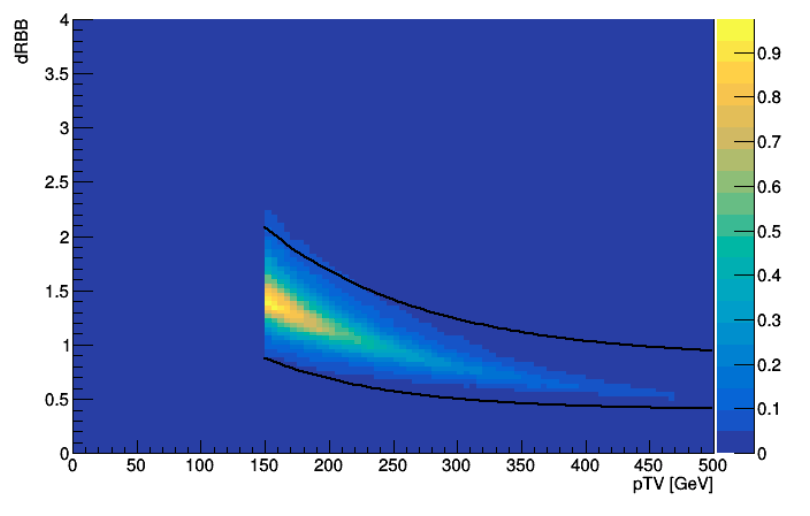
\includegraphics[width=0.505\linewidth]{1lep_qqWH_2tag_2jet.png}}
    \subfloat[]{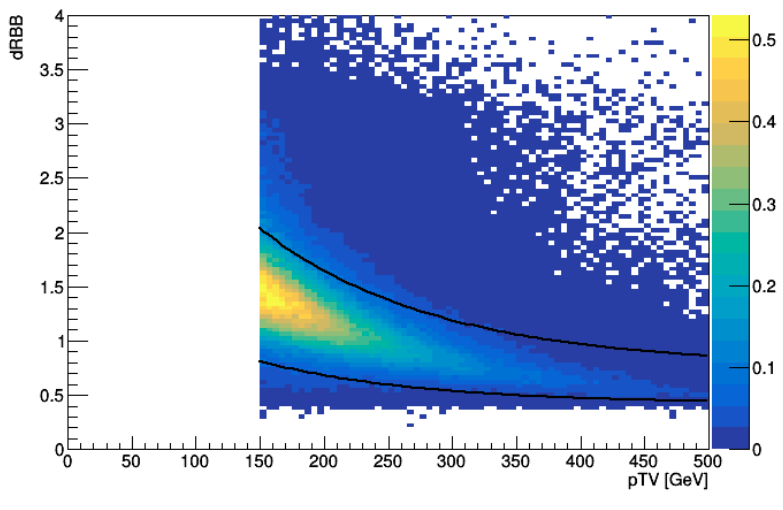
\includegraphics[width=0.49\linewidth]{1lep_qqWH_2tag_3jet.png}}\\
  \end{tabular}
  \caption{Signal distribution of $\Delta R$ between the two selected jets as
    function of $p_{T}^{V}$ in the 1--lepton channel are shown in the 2-tag 2-jet
    (a) and 2-tag 3-jet (b) categories. The black lines demonstrate the upper
    and lower continuous cuts used to categorise the events into the signal and
    control regions}
  \label{fig:drbb-crs}
\end{figure}